% !TEX root = ./problem.en.tex
\gdef\thisproblemauthor{}
\gdef\thisproblemdeveloper{}
\gdef\thisproblemorigin{}
\begin{problem}{膜術 Ena}
{standard input}{standard output}
{5 seconds}{512 MB}{}

這裡是兩個維度王國\newline
很久很久以前,巨龍突然出現,帶來災難,帶走了公主又消失不見\newline
王國十分危險,國王請來國內科技巨擎 -- 達拉崩巴 --,架設防禦設施\newline
達拉崩巴提出了使用防護膜的計畫阻止龍從空中入侵\newline
這種防禦膜架設在國內 N 根電線桿上,形成一條長長的折線\newline

\centerline{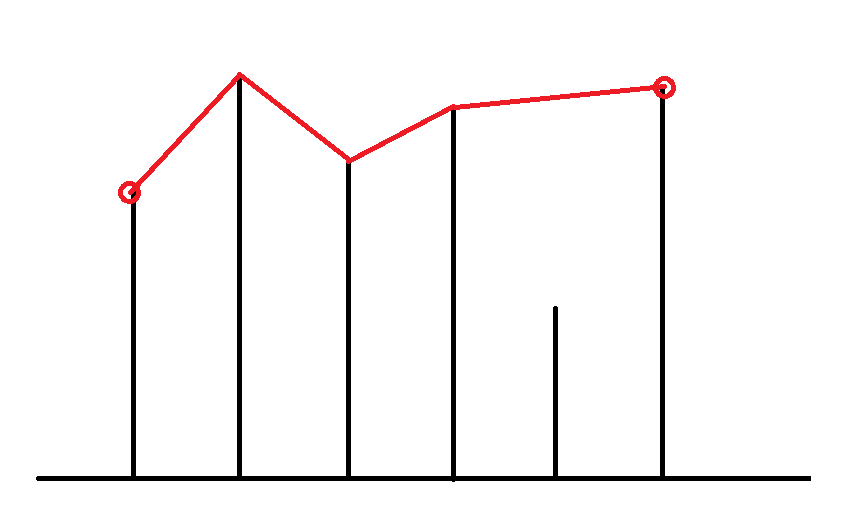
\includegraphics[height=15em]{./pics/D-1.png}}

因為是兩個維度王國,電線桿當然只能排成一直線\newline
而基於美學,這 N 根電線桿雖然高矮不同,但堅持相鄰兩根相隔一公尺\newline
\newline
因為由電線桿直接供電,所以盡可能希望與較多電線桿接觸\newline
\newline
然而,該材質限制不能轉折超過 $\pm D $ 度,否則會斷裂\newline
例如下圖中紅色 X 的地方\newline

\centerline{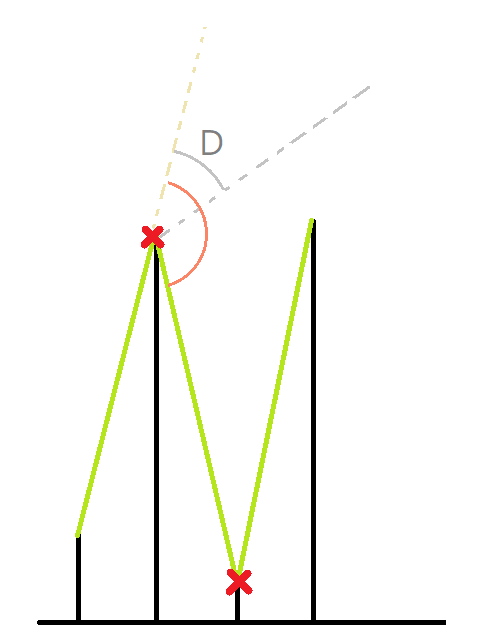
\includegraphics[height=25em]{./pics/D-2.png}}

而且也不能被某根電線桿刺穿\newline
例如:\newline

\centerline{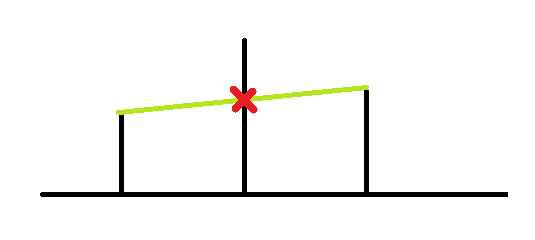
\includegraphics[width=25em]{./pics/D-3.png}}

因此有時候我們不得不放棄與某些電線桿接觸\newline
但為了包覆整個王國,一定要起於第一根、結束於最後一根\newline
\newline
\newline
你,達拉崩巴\newline
請找出能接觸到最多電線桿,能完整包住王國,而又不會斷裂的包膜方法吧!\newline

\InputFile

輸入 2 個正整數 $N$,$D$ ,表示有 $N$ 根電線桿,角度限制 $D$ 度 \newline
下一行有 $N$ 個正整數$h_1,h_2,...,h_n$,表示每根電線桿的高度(單位為公尺 )\newline

\begin{iofmt}
\begin{itemize}
	\item $2 \leq N \leq 10^4$
    \item $0 < D \leq 180$
    \item $0 <$ $h_i$ $\leq 1000 $
%	\item 所有可能的角度和 D 之間保證有 $10^{-6}$ 以上的差距 (無論是否會斷裂) 
    \item 有 3 分的測試資料 $ D = 180 $
	\item 有 10 分的測試資料 $N \leq 15$
	\item 有 45 分的測試資料 $N \leq 100$
\end{itemize}
\end{iofmt}

\OutputFile

輸出一個正整數,表示最多能跟幾根電線桿相接觸(含頭尾)\newline
要是沒辦法找出符合條件的包法,輸出 ``-1''(不含引號)\newline

\Examples

\begin{example}
 \exmpfile{./sample/PD-01.in.txt}{./sample/PD-01.out.txt}%
 \exmpfile{./sample/PD-02.in.txt}{./sample/PD-02.out.txt}%
 \exmpfile{./sample/PD-03.in.txt}{./sample/PD-03.out.txt}%
\end{example}

\Note

建議的計算角度方法: \\
對於二維向量$A=(x_1,y_1),\ B=(x_2,y_2)$ 求 $A$ 至 $B$ 的角度 $t \ ^{\circ}$ \\
$ t = (atan2(y_2,x_2) - atan2(y_1,x_1)) * 180.0 / \pi\ \ $\\
其中 atan2 在 C++ 的 <cmath>,以及 C 的 <math.h> 可以找到\\
$\pi$ 則以 acos(-1.0) 為準
\end{problem}
